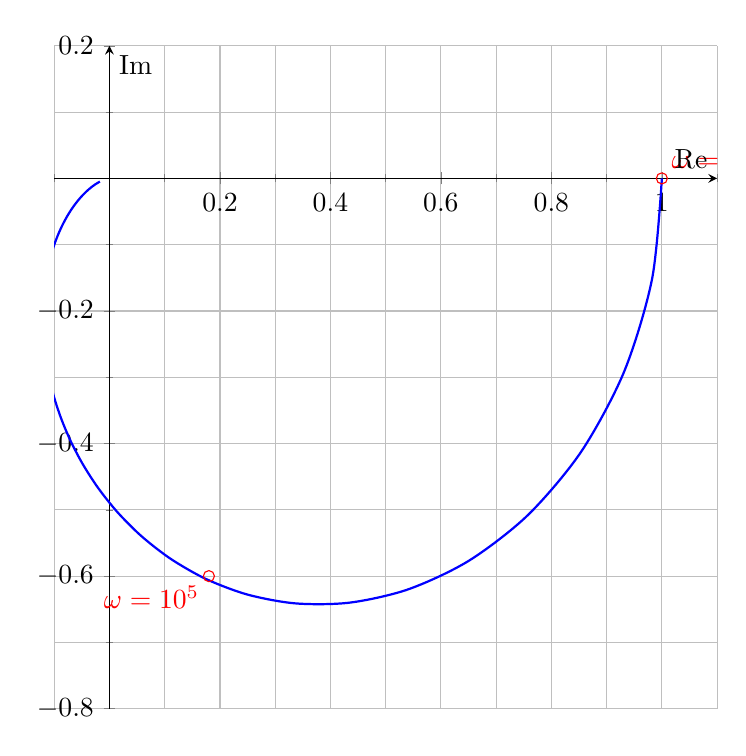
\begin{tikzpicture}
    \begin{axis}[
        xlabel={Re},
        ylabel={Im},
        grid=both,
        width=10cm,
        height=10cm,
        xmin=-0.1, xmax=1.1,
        ymin=-0.8, ymax=0.2,
        axis lines=middle,
        minor tick num=1,
        samples=100,
    ]
        \addplot[blue, thick, smooth, domain=0:10] ({
            (1 - x^2 * 0.5465) / ((1 - x^2 * 0.5465)^2 + x^2 * (1.5106)^2)
        }, {
            (-x * 1.5106) / ((1 - x^2 * 0.5465)^2 + x^2 * (1.5106)^2)
        });
        
        \addplot[only marks, red, mark=o] coordinates {(1,0)} node[above right] {$\omega=0$};
        \addplot[only marks, red, mark=o] coordinates {(0.18,-0.6)} node[below left] {$\omega=10^5$};
    \end{axis}
\end{tikzpicture}
